\RequirePackage{fixltx2e} %This package in CTeX is not compatible with revtex4-1
\documentclass[aps,pre,12pt,preprint,onecolumn,showpacs,showkeys]{revtex4-1}
\usepackage{ctex}
\usepackage{mathtools,mathrsfs}
\usepackage{multirow}
\usepackage{setspace,dcolumn}
\usepackage{hyperref}
\usepackage{graphicx,psfrag,epsfig}
\usepackage[font=small,format=plain,labelfont=bf,textfont=it,justification=centering,singlelinecheck=false]{caption}
\usepackage{amsmath,amsfonts,amssymb,amsthm,bm,upgreek}
\usepackage{geometry}
\usepackage[mathscr]{eucal}
\usepackage{caption}
\usepackage{subcaption}
\hypersetup{colorlinks=true}
\geometry{top=2.54cm,bottom=2.54cm,left=3cm,right=3cm}
\renewcommand\appendixname{附录}
\renewcommand\abstractname{}%摘要
\renewcommand\tablename{表}
\renewcommand\figurename{图}
\makeatletter
\def\@pacs@name{\songti\zihao{-4}{\bf PACS码:}}
\def\@keys@name{\songti\zihao{-4}{\bf 关键词:}}
\def\Dated@name{日期:}
\def\Received@name{\zihao{-5}{接收} }
\def\Revised@name{\zihao{-5}{修订} }
\def\Accepted@name{\zihao{-5}{采纳} }
\def\Published@name{\zihao{-5}{发表} }
\makeatother
\linespread{1.3}
\renewcommand{\labelenumi}{\alph{enumi}.}
\leftmargini=20mm
\def \d {\mathrm d}
\def \degree {^\circ}
\def \V {\bm{V}}
\def \degC {^\circ \mathrm{C}}

\begin{document}
\title{\bf\heiti\zihao{3}电子自旋共振\vspace{15mm}}
\author{\fangsong\zihao{4}邵智轩\vspace{2mm}}
\affiliation{\songti\zihao{-4}学号:1400012141\vspace{2mm}}
\date{\today}
%\pacs{02.10.Yn, 33.15.Vb, 98.52.Cf, 78.47.dc}
\keywords{微波,自旋磁矩,共振跃迁,反射式谐振腔,$g$因子,弛豫时间}
\email{shaozhixuansh@pku.edu.cn; (86)13381350619}

\begin{abstract}
\vspace{10mm}
\begin{spacing}{1.5}
\songti\zihao{-4}
    本实验学习了电子自旋共振的(ESR)的原理。了解观察电子自旋共振波谱的微波系统,熟悉一些微波器件的使用方法及反射式谐振腔的工作特性;通过对DPPH自由基的电子自旋共振谱线的观察,了解电子自旋共振现象及共振特征。学会测量共振场、自由基$g$因子、共振线宽和弛豫时间,加深对电子自旋共振知识的理解。

\end{spacing}
\end{abstract}
\maketitle
\songti\zihao{-4}

\section{引言}
    电子自旋共振(ESR)或电子顺磁共振(EPR),是指有未成对电子的原子、离子或分子的顺磁性物质,在恒定磁场作用下对微波能量发生的共振吸收现象。如果共振仅仅涉及物质中的电子自旋磁矩,就称为电子自旋共振;但一般情况下,电子轨道磁矩的贡献是不能忽略的,因而又称为电子顺磁共振。电子自旋共振研究的主要对象是化学自由基、过渡金属离子和稀土离子及其化合物、固体中的杂志、缺陷等。通过对这类顺磁物质的电子自旋共振波谱的观测,可以了解这些物质中未成对电子状态及其周围环境方面的信息,因而是探索物质微观结构的重要工具。

\section{原理}
    \subsection{电子自旋共振}
    电子的总磁矩与总角动量的数值具有如下关系:
    \begin{equation}
        \mu=g \frac{e}{2 m_e} P
    \end{equation}
    又可写成:
    \begin{equation}
        \mu =\gamma P
    \end{equation}
    比例系数$\gamma=g \frac{e} {2 m_e}$称为旋磁比。

    电子自旋磁矩在外加恒定磁场下会发生Lamour进动,如果在外加磁场的同时,沿垂直外磁场方向加一个微波场,当微波的频率与磁矩进动的频率一致时,微波能量将被强烈吸收,即称为共振现象。被吸收的能量为磁矩进动提供克服阻尼的动力,使进动能够持续下去。从量子力学的观点来看,共振是指在某一特定的外磁场作用下,微波场与磁矩间相互作用而发生的塞曼能级间的感应跃迁。在外磁场,能级劈裂成两个,它们的差值与外加恒定磁场成正比:
    \begin{equation}
        \Delta E= E_a - E_b =\frac{1}{2}g \mu_B H- (-\frac{1}{2}g \mu_B H)=g \mu_B H
    \end{equation}
    如果在自由基分子所在的恒定磁场区加一个同恒定磁场垂直的微波场,它的频率为$\nu$,使得微波量子的能量正好等于上述能级差,
    \begin{equation}
        h \nu = g \mu_B H, \quad 2\pi \nu=\gamma H \label{eq:resonance_cond}
    \end{equation}
    那么,电子在相邻的能级之间将发生\textbf{磁偶极共振跃迁}。

    为了满足共振条件(\ref{eq:resonance_cond}),实验中可以采用固定微波频率改变外磁场的扫场方式。

    \subsection{线宽、弛豫作用}
    实际的吸收谱线不是无限窄,而是有一定宽度的,这一宽度是自旋-自旋耦合与自旋晶格耦合共同作用的结果。线宽的存在表明,当发生电子顺磁共振时,顺磁系统达到新的热平衡是需要一个弛豫过程的。弛豫过程越快,线宽就越宽。因此线宽可以看作是弛豫强弱的度量。

    记线宽为$\Delta H$,弛豫时间为$T$,则有
    \begin{equation}
        \Delta H= \frac{1}{\gamma T}
    \end{equation}
    对于稳定的自由基,$T\approx T_2$,$T_2$为自旋-自旋弛豫时间(横向弛豫时间)。对于洛伦兹线型,从布洛赫方程可以得到:
    \begin{equation}
        T_2 =\frac{2} {\gamma \Delta H}\label{eq:time}
    \end{equation}

\section{实验内容}
\begin{figure}[ht]
    \centering
    \includegraphics[width=120mm]{equipment}
    \caption{\label{fig:equipment}%
    微波电子顺磁共振实验装置}
\end{figure}
    \subsection{测量腔的谐振频率$f_0$}
    测量时使固态源工作于\textbf{等幅}工作状态,数字式电压表读数为12V。调节振荡器上的测微头,使振荡器的输出频率约为9000 MHz,这时检测到较大的检波电流。通过1臂上的单螺调配器调节阻抗,使检波电流逐渐减小,直至检波电流接近于0,表明1臂与2臂的负载已经对称,桥路达到平衡,反射式谐振腔发生谐振,微波信号与谐振频率$f_0$一致。

    用波长计测得此时的频率为
    \begin{equation}
        f_0=9014 \mathrm{MHz}\label{eq:freq}
    \end{equation}
    在以下测量中,保持微波频率(\ref{eq:freq})不变。

    \subsection{观察DPPH自由基电子自旋共振信号,测量相应的自旋共振场$H_0$,由此确定自由基的$g$因子和旋磁比}

    \begin{figure}[ht]
        \begin{minipage}{.5\textwidth}
            \centering
            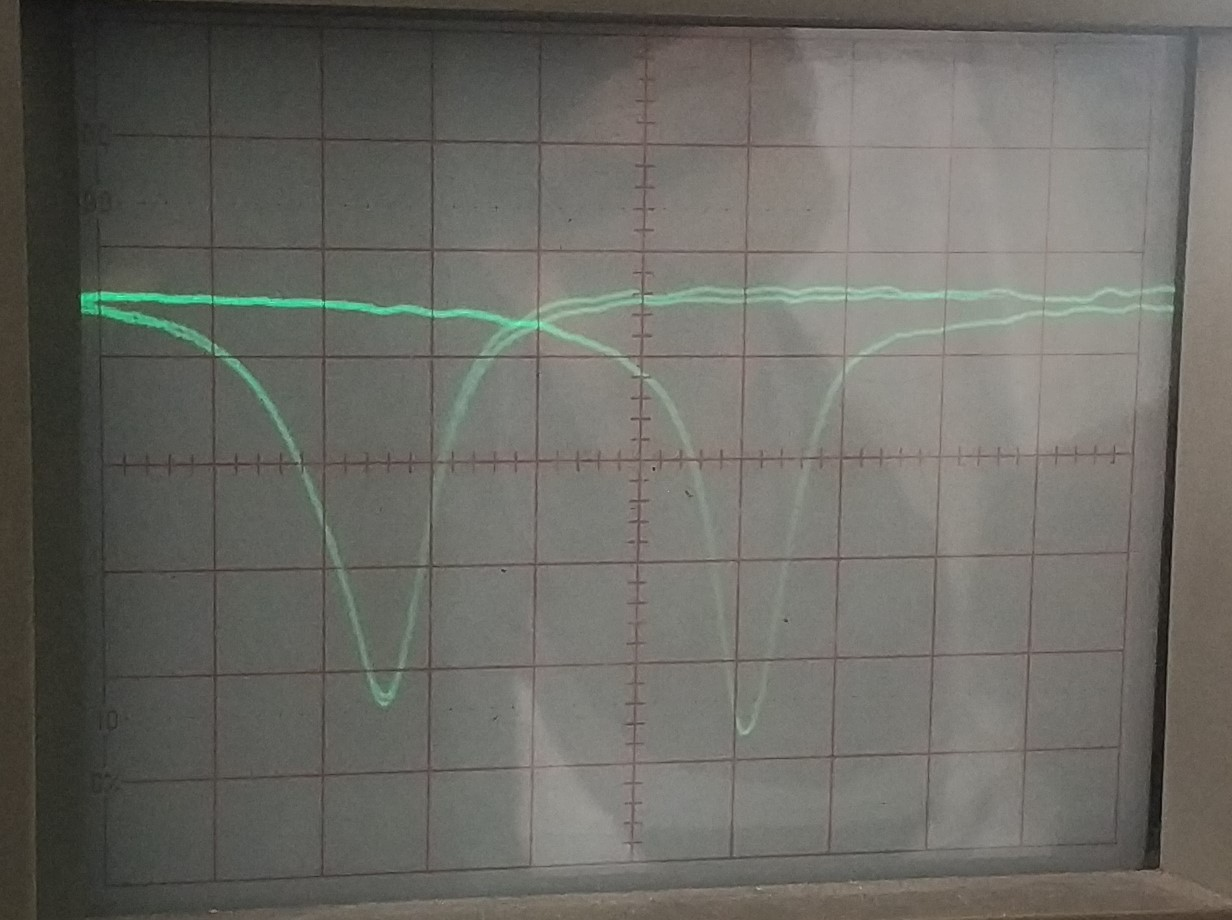
\includegraphics[width=75mm]{fig_1}
            \caption{\label{fig:1}%
            X-Y显示下电子自旋共振信号}
        \end{minipage}%
        \begin{minipage}{0.5\textwidth}
            \centering
            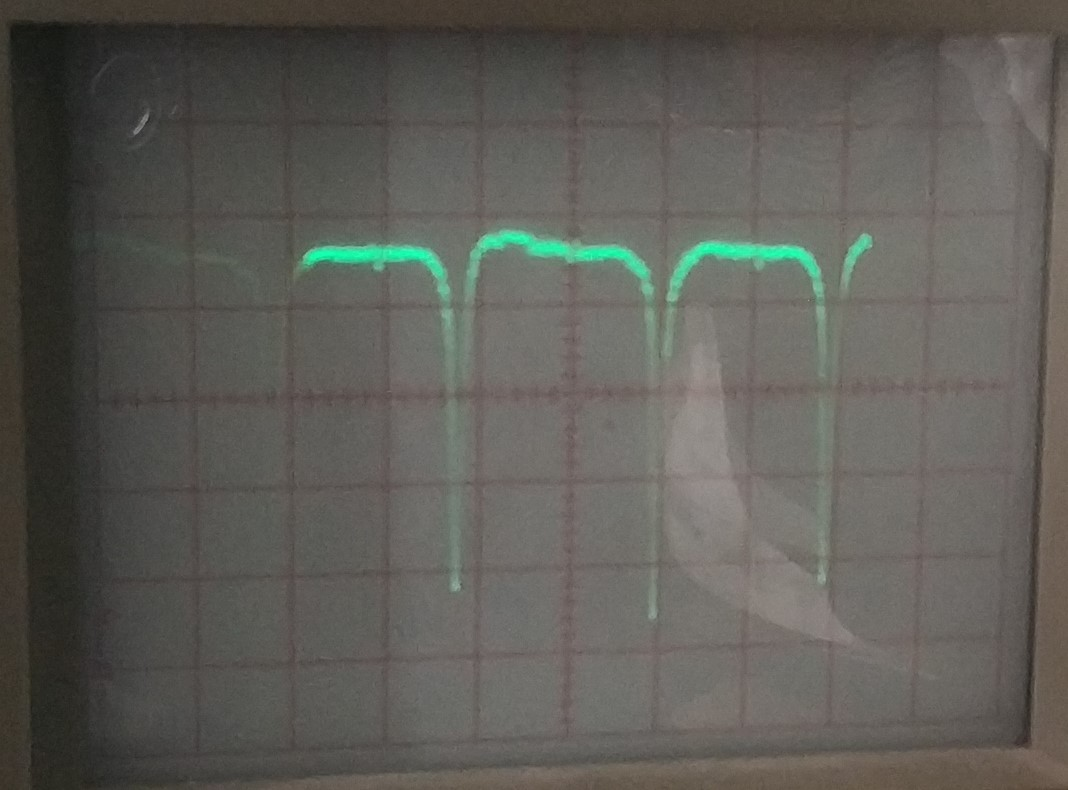
\includegraphics[width=75mm]{fig_2}
            \caption{\label{fig:2}%
            扫描显示下电子自旋共振信号}
        \end{minipage}
        
    \end{figure}

    开启“扫场”,调节“磁场”旋钮,使励磁电流逐渐增大到1.73A附近,示波器上出现共振信号,如图\ref{fig:1}所示。

    将示波器调至扫描状态,观察到的信号如图\ref{fig:2}所示。调节磁场旋钮,使各共振信号成等距状态,此时对应的磁场就是共振场$H_0$,用霍尔磁场计测量磁场大小为:
    \begin{equation}
        H_0 = 3230 \mathrm T
    \end{equation}
    由此可以计算出旋磁比$\gamma$:
    \begin{equation}
        \gamma=\frac{2 \pi f_0}{H_0}=1.7535 \times 10^{11} \mathrm T ^{-1}
    \end{equation}
    以及$g$因子:
    \begin{equation}
        g=1.9939
    \end{equation}
    与理论值($g=2.0023$)吻合。

    \subsection{测量共振线宽$\Delta H$与弛豫时间$T_2$}\label{biaoding}
    将示波器置于X-Y显示。先对磁场进行标定。将磁场计置于样品附近固定位置,固定扫场大小(比如调至最小),调节“磁场”旋钮使某一个固定点(比如峰值的对应点)左右移动,测量相应的磁场变化量和移动格数,测量三次取平均值。我的标定结果为:0.0025T/50小格,即0.00005T/小格。线宽(半高宽)为7小格,得
    \begin{equation}
        \Delta H \approx 3.5 \times 10^{-4} \mathrm T
    \end{equation}
    代入(\ref{eq:time})算得$T_2$:
    \begin{equation}
        T_2 = \frac{2} {\gamma \Delta H}\approx 3 \times 10 ^{-8} \mathrm s
    \end{equation}

\section{结论}
    本实验学习了电子自旋共振的(ESR)的原理。了解观察电子自旋共振波谱的微波系统,熟悉一些微波器件的使用方法及反射式谐振腔的工作特性;通过对DPPH自由基的电子自旋共振谱线的观察,了解电子自旋共振现象及共振特征。测量了谐振频率$f_0=9014 \mathrm{MHz}$、自由基$g$因子$g=1.9939$。还大致估计了共振线宽$\Delta H \approx 3.5 \times 10^{-4} \mathrm T $和横向弛豫时间$T_2\approx 3 \times 10 ^{-8} \mathrm s$。

\section{致谢}
    感谢王常生老师对实验的悉心指导,使我迅速掌握了电子自旋共振的原理,熟悉了微波器件的使用方法及反射式谐振腔的工作特性。尤其是王老师主张让我们自己多琢磨琢磨,要敢于尝试,勤于思考,这种精神让我受益匪浅。
    
\begin{thebibliography}{}
\bibitem{Book} 吴思诚, 荀坤. 近代物理实验(第四版). 北京:高等教育出版社, 2015
\end{thebibliography}
\end{document}